%\documentclass[3p,twocolumn]{article}
\documentclass[12pt]{article}

\usepackage{graphicx}
\usepackage{color}
\usepackage{url}
\usepackage{ifpdf}
\usepackage{hyperref}
\usepackage{xspace}
%\usepackage[draft]{pdfdraftcopy}

\setlength\parskip{-0.015em}
\setlength\parsep{-0.15em}

\newenvironment{shortlist}{
	\vspace*{-0.85em}
  \begin{itemize}
 \setlength{\itemsep}{-0.3em}
}{
  \end{itemize}
	\vspace*{-0.6em}
}

\usepackage{fullpage}
%\usepackage[top=tlength, bottom=blength, left=llength, right=rlength]{geometry} %http://en.wikibooks.org/wiki/LaTeX/Page_Layout
%\usepackage[margin=1in, paperwidth=5.5in, paperheight=8.5in]{geometry}

\usepackage{fancyhdr}
\setlength{\headheight}{16.0pt}
\pagestyle{fancy}
\headheight = 0pt
\headsep    = 25pt
\fancyhf{}
%\fancyhead[OC]{\bf {\it \footnotesize{Jha et al: A Case for SAGA as an Access Layer for DCI}}}

\newif\ifdraft
\drafttrue
\ifdraft
 \newcommand{\amnote}[1]{  {\textcolor{magenta} {***AM: #1}}}
 \newcommand{\jhanote}[1]{ {\textcolor{red}     {***SJ: #1}}}
 \newcommand{\olenote}[1]{ {\textcolor{blue}    {***OW: #1}}}
\else
 \newcommand{\amnote}[1]{}
 \newcommand{\jhanote}[1]{}
 \newcommand{\olenote}[1]{}
\fi

\newcommand{\dn}{\vspace*{0.33em}}
\newcommand{\dnn}{\vspace*{0.66em}}
\newcommand{\dnnn}{\vspace*{1em}}
\newcommand{\uppp}{\vspace*{-1em}}
\newcommand{\upp}{\vspace*{-0.66em}}
\newcommand{\up}{\vspace*{-0.33em}}
\newcommand{\shift}{\hspace*{1.00em}}

\newcommand{\T}[1]{\texttt{#1}}
\newcommand{\I}[1]{\textit{#1}}
\newcommand{\B}[1]{\textbf{#1}}
\newcommand{\BI}[1]{\B{\I{#1}}}
\newcommand{\F}[1]{\B{[FIXME: #1]}}
\newcommand{\TODO}[1]{\textcolor{red}{\B{TODO: #1}}}

\begin{document}

\title{Towards a Scalable Architecture for Deep Sequencing Analytics}

\author{Joohyun Kim$^{1}$, Sharath Maddineni$^{1}$, Shantenu Jha$^{*1,2}$, \\
  \small{\emph{$^{1}$Center for Computation \& Technology, Louisiana State University, USA}}\\
  \small{\emph{$^{2}$Department of Computer Science, Louisiana State University, USA}}\\
  \small{\emph{$^{*}$Contact Author \texttt{sjha@cct.lsu.edu}}}
  }


\maketitle

\section*{Abstract}

We investigate the use of distributed computing environments, a
production HPC grid and a cloud environment for the genome-wide
mapping with BFAST.  The main goal of this work is to understand the
characteristics of these two distributed computing environments and
compare and contrast their strengths and suitability to support the
computational requirements of deep sequencing.
% regarding computational requirements of the target bioinformatics
% application whose 

We investigate two model genomes -- human genome and a microbe,
Burkerholderia Glumae, that might represent a eukaryote and a
prokaryote system.  The computational complexity of execution of bioinformatics calculation, mapping with BFAST, 
depends upon the size of a reference genome, the data size of short
reads from high-throughput technologies of the Next Generation
Sequencing platforms, and their biological genome contexts such as distinctive differences between prokaryotes vs eukaryotes.

The two distributed environments, the Louisiana Optical Network
Initiative (LONI) grid and a Cloud system from the FutureGrid, were
used primarily focusing on different and unique challenges in HPC and
Cloud computing conditions.

The time to completion are analyzed by comparing advantages as well as
limitations of each distributed computing infrastructure in
conjunction with distinctively different two different genome systems.
With our results, we discuss the importance of an effective runtime
environment that facilitates a rapid development of
cyberinfrastructure of distributed computing resources and supports
optimized execution patterns for a target scientific application, in
particular, of the data-intensive genome-wide analysis.


\section{Introduction}

% \bibliographystyle{plain}
% \bibliography{egi-white-paper}

High-throughput sequencing techniques including deep sequencing
approaches such as ChIP-seq and RNA-seq have changed biological
sciences and biomedical research dramatically with their genome-wide
information.  Consequently, the need of computational methods for
resolving new challenges and requirements of processing and analyzing
genome sequencing data is increasingly taken into account
indispensable for successful outcomes but the development of
infrastructure and required software remain major challenges.  The
complexity of biological information as well as the size of relevant
genomics data as well as difficulty of the utilization of
heterogeneous distributed computing resources constitute such
challenges.

We primarily focus on the mapping process of short reads from NGS
platforms against a reference genome.

\jhanote{we want to present a strawman of an architecture based upon
  requirements and a reference implementation of the architecture} In
this work, we present our work on the infrastructure development for
the use of High Performance Computing (HPC) grids and Cloud
environment for genome-wide analysis.

The development of an efficient runtime environment, which is the key part of our development, requires an understanding of biological information that the target scientific application aims to produce as well as of execution patterns and scalability of the computing resources of interest to be deployed.  First, we note that in general, genome-wide mapping procedure is an good example of data-intensive scientific applications and can be efficiently carried out with parallel or concurrent executions if there exist ways of data fragmentation with intact biological information.  For example, a reference genome is likely to be composed of many chromosomes or plasmids, and thus mapping on each chromosomes and plasmids can be executed separately.  The challenge, however, is that the way of data fragmentation, and thus system configuration for required parallel/concurrent runs should be considered the characteristics of system environment. Those characteristics differ distinctively between a HPC grid and a Cloud and also vary with a specific target system in each class.  

\section{Applications: An Overview}
First, for genome-wide mapping procedure with a mapping application, BFAST, we need to carry out several stages that include a step for genome indexing with a reference genome and for match of short reads sequencing data against a indexed reference genome.  In this work, we focus on match.   The overall workflow that explains the target calculation, match, and other pre-processing steps is illustrated in Fig.~\ref{fig:workflow-bfast}. 


\begin{figure}
 \centering
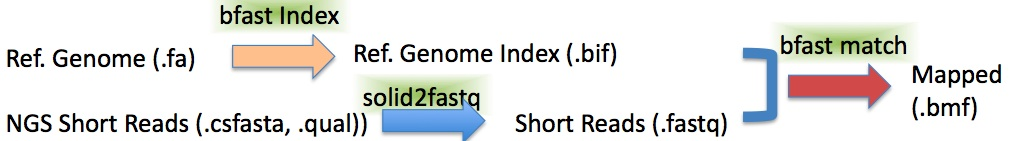
\includegraphics[scale=0.35]{bfast-mapping.jpg} 

\caption{\small Overall workflow for mapping procedure using BFAST for ABI SOLiD sequencing data is illustrated with Bfast commands and the associated module, solid2fastq.  In this work, we focus on the step for match (red arrow).  Note that initially a reference genome stored with a fasta file format (.fa) and NGS sequencing data, whose file format varies depending upon NGS platform), are converted into index files (xxx.bif) and fastq files, respectively.  }
  \label{fig:workflow-bfast} \end{figure}


In Table~\ref{table:two-genomes}, we summarize the raw data sizes for two genomes and the information.  Note that the number of required concurrent tasks, $N$, for match is decided by the number of indexed files (xxx.bif), $N_i$, and the number of files for the sequencing data (xxx.fastq), $N_s$, such that $N = N_i \times N_s$.   The decision could result in the optimized time-to-solution, and to this end, importantly needs the information about the specification of available computing environments such as the available number of cpus, accessible memory size, and the size of data storage for each task as well as biological information such as the number of chromosomes.    


\jhanote{Joohyun: Please organize each description addressing each of
  the following points: (i) Brief outline of the scientific problem,
  (ii) What are the challenges, (iii) estimates of volumes of data
  involved, distributed or not?, number of tasks, are they coupled or
  uncoupled -- what is the level of coupling between tasks?}

\begin{table}
\begin{tabular}{|c|cc|} 
\hline 
Genome Species & Human  & Burkerholderia Glumae  \\ \hline
 Type of Genome Analysis &  Exome  & Whole Genome Resequencing \\
  Sequencing Platform & ABI SOLiD  &  Illumina GA2 \\
  Num. of nucleotides in a Reference Genome (in bp) &  3 G & 7.3 M \\
 Size of Sequencing Data (.fastq) (in Byte) & 8.7G & 5.4 G \\

\hline
\end{tabular} \caption{Specification of target genomes and sequencing data from Next Generation Sequencing (NGS) platforms.}
 \label{table:two-genomes} 
\end{table}

 \begin{table}
 \begin{tabular}{|c|cc|} 
 \hline 
Distributed Environment &  HPC Grid &  Cloud \\ \hline
System  &  Louisiana Optical Network Initiative & FutureGrid \\
Name &  QB/Eric   &  INDIA/SIERRA \\
 \hline
 \end{tabular}
\caption{Specification of two distributed environments}
\label{table:two-systems} 
\end{table}
 
\section{Existing Solutions: Limitations and Challenges}

\jhanote{Here we need to define what solutions are currently employed, what works well
  what doesn't}

\section{Runtime Environment}

The DARE framework, comprising an open source Web application, Pylons
and the runtime environment for distributed scientific applications,
was employed for this work.  The framework enables us to develop a
lightweight, extensible, full-fledged science gateway effectively in
which the runtime environment built upon SAGA and BigJob abstraction
manages efficiently distributed computing-driven execution patterns of
target scientific applications.

There are two steps for the BFAST implementation. First step is to prepare read files in the 
fastq format and in the second step we run matching using BFAST with the prepared read files.
 We can generate as many number of read files as we want in the first step in the first step
 but the second step could be scaled with more number of tasks. Because the number tasks 
 in the second step is determined by the number read files we prepare in the first step. We 
 can generate as many number of read files as we want in the first step. We can use as many resources/machines 
 in this step as the tasks are not coupled to each other but the problem is we need the transfer the appropriate read file
in to the respective resource.

37 tasks for the second step was chosen arbitrarily to show the scaling  and to find the performance 
difference with concurrent tasks in the second step. So 37 read files should be prepared in the
 first step by setting the parameters accordingly.

We use SAGA-BigJob to implement the above two steps on grids and clouds and 
the architecture remains BigJob remains same for both grids and clouds. All the first 
step jobs and second step jobs are defined as subjobs in the BigJob. At first only 
one job is submitted ie  preparing the read files and the jobs in the second step are not submitted
until the first job is done. Once the Read files are prepared the 37 subjobs are submitted in to 
job queue of the Bigjob. Number of concurrent subjobs that can be processed depending 
on the available cores that are requested in the BigJob.
  
In the Grid implementation first all the data required in the steps was transferred to machine's  work 
directory where we want to start the BigJob. The Bfast was installed in the home directory and the
executables path for job description of subjobs was given accordingly.

In the cloud implementation all the data required was transferred into the walrus because of the data size limitation of the storage space in the
running VM. Multiple VM's can be started at once and the data in the walrus is mounted onto all the running VM
while booting the Virtual Machine. Thus all the VM can have access to data and can process concurrently





\end{document}

